\subsubsection{Dinâmica do manipulador}\label{sec::dinamica}
A dinâmica de um manipulador robótico é a análise de velocidades, acelerações e
torques das juntas. Para esta análise, assume-se que o efetuador, pistola de
revestimento, possui velocidade 40m/min constante em todos os pontos amostrados
da pá. Como velocidades e acelerações exigem a computação de derivadas, é
realizada uma melhor discretização da pá da turbina, na qual o passo de
amostragem é menor e um filtro garante espaçamento uniforme dos pontos de 10 mm.
Para um lado da pá, são amostrados, portanto, 130 mil pontos.

Para cada ponto amostrado da pá, faz-se a análise cinemática e são armazenados
os pontos que são possíveis de serem revestidos, como na
seção~\ref{sec::cinematica}, isto é, são armazenados os pontos que possuem
solução de cinemática inversa. Posteriormente, para cada ponto revestido, é
criado um conjunto contendo seus 8 pontos vizinhos através de um algoritmo k-d
tree, como na figura~\ref{fig::pontosdin}, onde $p_r$ é o ponto de referência a
ser analisado dinamicamente e os pontos ${p_1,p_2,q_1,q_2,r_1,r_2,s_1,s_2}$ são auxiliares
para o estudo. 

\begin{figure}[h!]	
	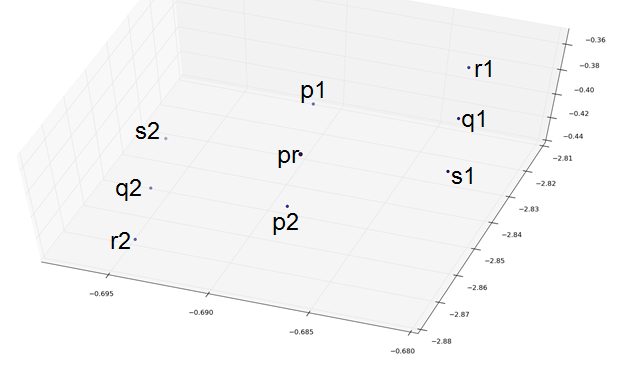
\includegraphics[width=\columnwidth]{figs/dinamica/pontosdinamica.png}
	\caption{Pontos exemplo amostrados da pá.}
	\label{fig::pontosdin}
\end{figure}

%As soluções de cinemática inversa (ângulos das juntas do robô)
%$\Theta_r
%=
%{\theta_{p_r},\theta_{p_1},\theta_{p_2},\theta_{q_1},\theta_{q_2},\theta_{r_1},\theta_{r_2},\theta_{s_1},\theta_{s_2}}$
As velocidades angulares das juntas são calculadas a partir da cinemática
diferencial. Para isso, usa-se o cálculo da matriz jacobiana ($J$), que é a
diferenciação (derivadas parciais) da matriz de cinemática direta em função das
variáveis de junta \citep{sciavicco2000differential}. A velocidade linear do
efetuador ($\dot{X}$) e o jacobiano são conhecidos em cada ponto de referência, logo
podem-se calcular as velocidades das juntas do manipulador entre o ponto de
referência e cada ponto auxiliar: $\dot{X} = J\dot{q}\Rightarrow
J^+\dot{X}=\dot{q}$, onde $J^+$ é a pseudo inversa Moore-Penrose de $J$.

As velocidades angulares são $\Omega_r
=
\{\omega_{p_r,p_1},\omega_{p_r,p_2},\omega_{p_r,q_1},\omega_{p_r,q_2},\omega_{p_r,r_1},\omega_{p_r,r_2},\omega_{p_r,s_1},\omega_{p_r,s_2}\}$,
onde $\omega$, $\omega\in\Omega_r$, é um vetor $n \times 1$, e $n$ é o número de
juntas do robô. As velocidades dos ângulos das juntas é uma informação importate para a
verificação da viabilidade das trajetórias do robô. Para o caso do robô
MH12, onde $\omega_{\textbf{max}}=\{220, 200, 220, 410, 410, 610\}^o/s$, por
exemplo, caso não haja $\omega\in\Omega_r$, tal que
$\omega\leq\omega_{\textbf{max}}$, não é possível realizar o revestimento do
ponto de referência $p_r$. Se $\exists \omega\in\Omega_r$ tal que
$\omega\leq\omega_{\textbf{max}}$, o ponto de referência é viável pela
cinemática inversa e pela cinemática diferencial, mas pode ser inviável ainda
pela análise dinâmica, que considera as acelerações, massas e forças do
conjunto.

As equações dinâmicas de um manipulador são também abordados em
\cite{sciavicco2000differential} e possuem duas abordagens bem conhecidas na
literatura: equações de Newton-Euler e equações de Lagrange. O ambiente OpenRave
utiliza o método de Newton-Euler para computar os torques das juntas (dinâmica
inversa): $\tau = M(q)\alpha + C(q,\omega)\omega + G(q) $, onde $\tau$ é o
vetor de torques das juntas, $M$ matriz de massas e momentos de inércia,
$\alpha$ é acelerações das juntas, $C$ matriz de Coriolis, $\omega$ é as
velocidades das juntas e $G$ o vetor de gravidade.

Para a formação da matriz $M$, é necessária a estimação de parâmetros do
manipulador. A estimação dos parâmetros pode ser realizada de maneira iterativa,
isto é, aplicam-se torques nas juntas e, pela resposta
do manipulador, estima-se a matriz \citep{slotine1988adaptive}; ou pelo CAD do
manipulador, por exemplo, pela utilização da ferramenta SolidWorks. Foi utilizado o método de estimação pelo CAD do
manipulador, visto que os manipuladores ainda estavam em estudo e não foram
adquiridos, além disso houve facilidade de aproximar os parâmetros já que o CAD
fornecido pelo fabricante é bem detalhado. 

A aceleração angular, $\alpha$, é necessária para a computação dos torques,
$\tau$. O método analítico para cálculo da aceleração angular das juntas é
através da derivada da equação da cinemática diferencial:
$\ddot{X}=\dot{q}^TH\dot{q}+J\ddot{q} \Rightarrow
\ddot{q}=J^+(\ddot{X}-\dot{q}^TH\dot{q})$ ou
$\alpha=J^+(a-\omega^TH\omega)$, onde $H$ é a matriz Hessiana, isto é, derivada
parcial da matriz jacobiana $J$ \citep{hourtash2005kinematic}. 

Com a informação dos ângulos, velocidades e acelerações das juntas, momentos
de inércia e massa dos elos, o OpenRave calcula a dinâmica inversa através do
método Newton-Euler, obtendo-se os torques. Para cada ponto de referência, há quatro direções
(trajetórias) possíveis amostradas que o efetuador pode percorrer:
$\{(p_1,p_r,p_2),(q_1,p_r,q_2),(r_1,p_r,r_2),(s_1,p_r,s_2)\}$, logo quatro
ângulos, velocidades e acelerações de juntas, portanto são obtidos quatro
possíveis vetores de torques:
$T=\{\tau_{rp},\tau_{rq},\tau_{rr},\tau_{rs}\}$. E, especificamente para o
caso do manipulador MH12, os valores dos torques devem ser inferiores aos
estabelecidos pelo datasheet:
$\tau_{\textbf{max}}=\{-,-,-,22,22,9.8\}\textbf{Nm}$, logo se $\exists \tau\in
T$, tal que $\tau\leq\tau_{\textbf{max}}$, então há uma trajetória viável.

As figuras~\ref{fig::wgeo}, ~\ref{fig::wcin} e ~\ref{fig::wdin} representam a
evolução das análises do manipulador, de um nível mais simples a um nível mais
complexo de detalhamento, o qual avalia velocidades, acelerações e torques das
juntas do manipulador. Ainda deverá ser executada a análise de manipulabilidade
que avalia o sistema de controle do manipulador. Esta análise é importante para
o planejamento de trajetórias do manipulador e para o cálculo das posições
viáveis da base para uma operação completa.



\begin{figure}[h!]	
	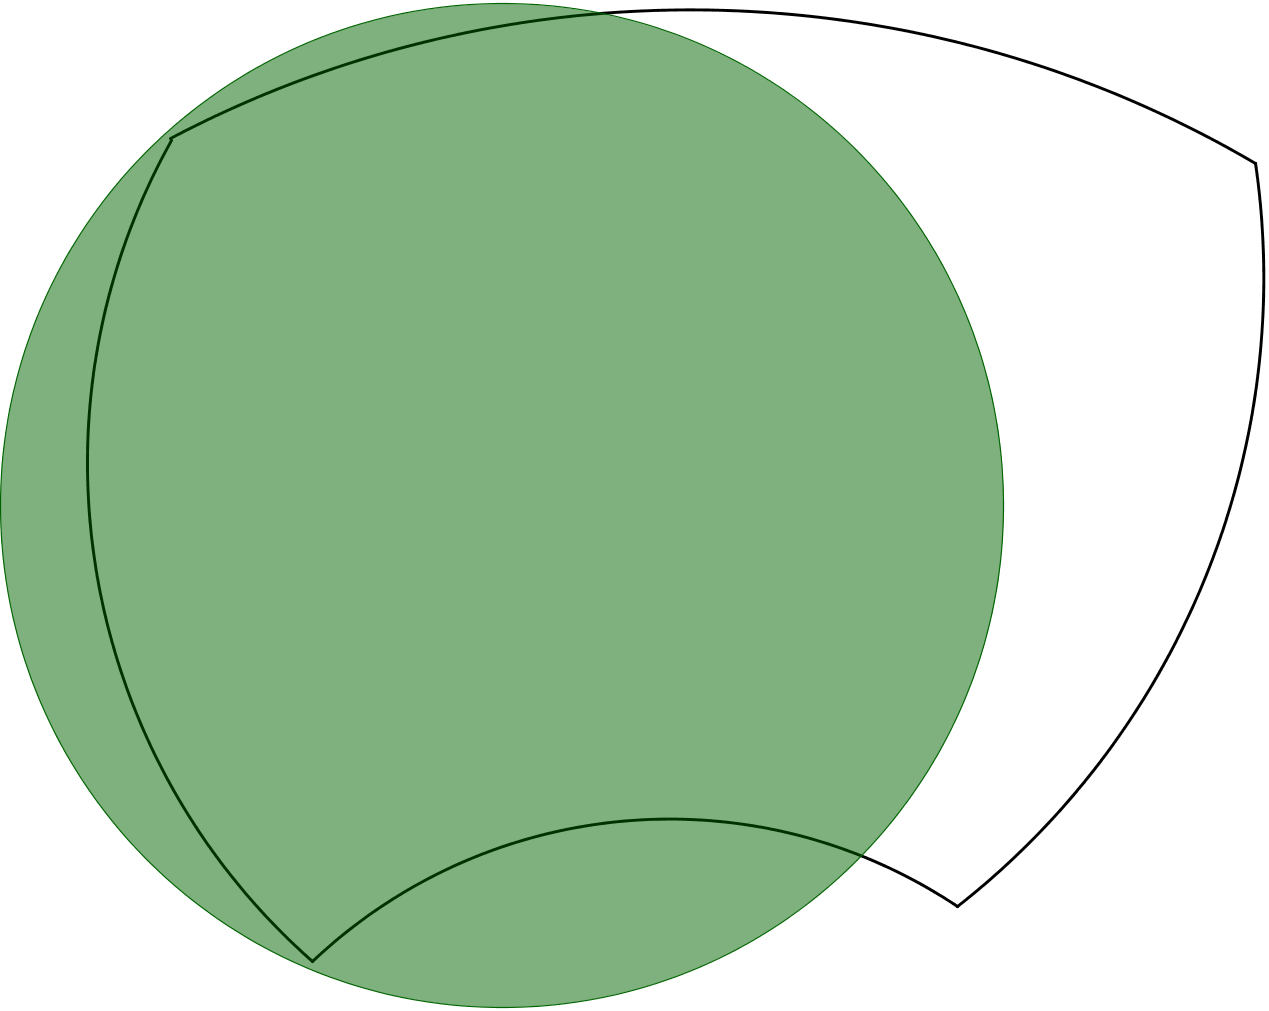
\includegraphics[width=\columnwidth]{figs/dinamica/workspaceGeometrico.png}
	\caption{Área em verde representa a cobertura do revestimento executada pelo
	manipulador, utilizando a abordagem puramente geométrica.}
	\label{fig::wgeo}
\end{figure}

\begin{figure}[h!]	
	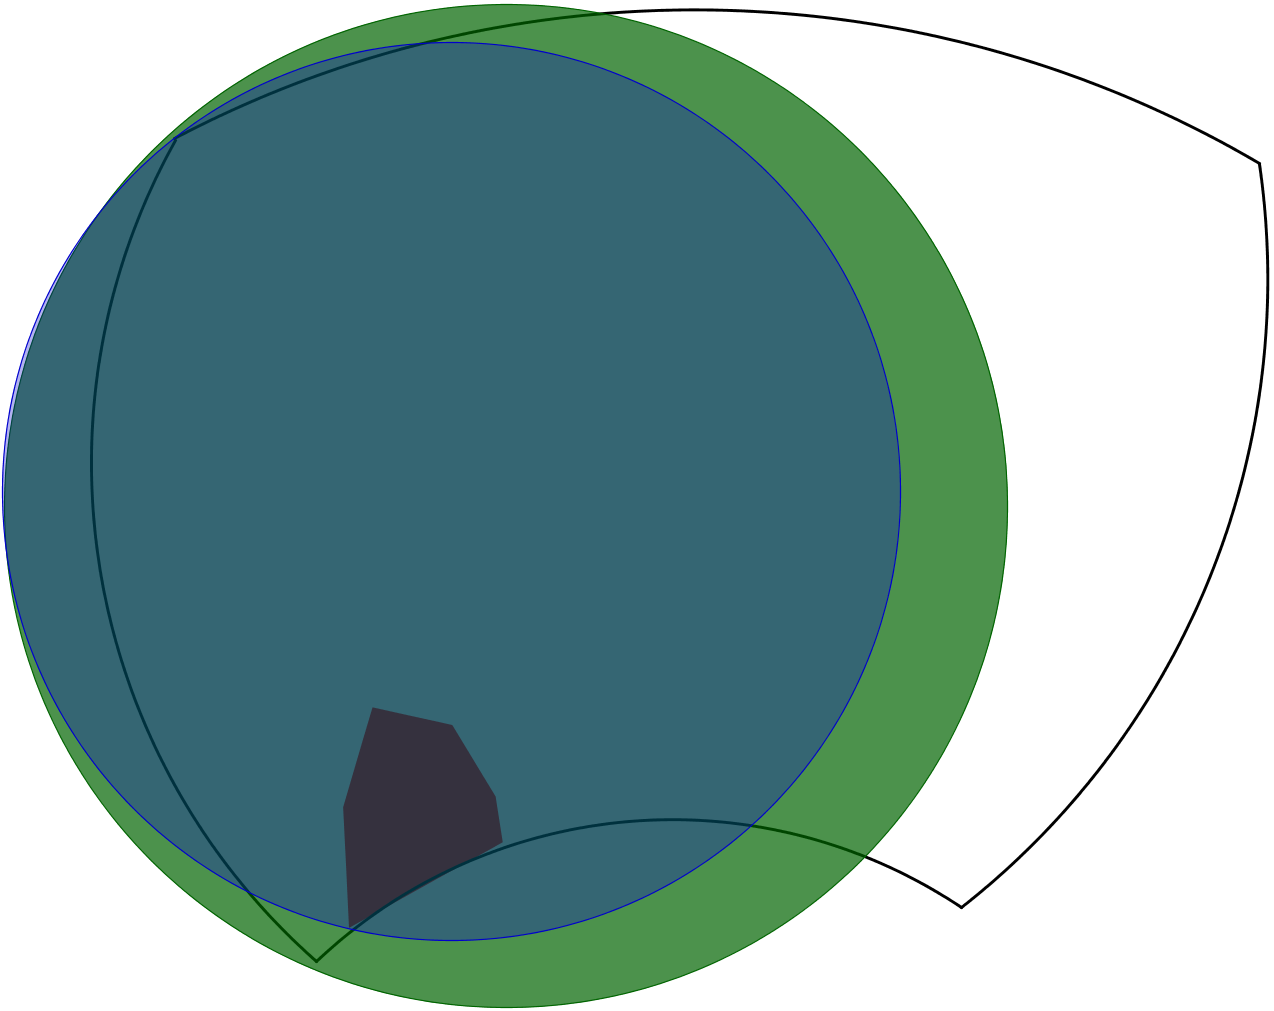
\includegraphics[width=\columnwidth]{figs/dinamica/workspaceCinematica.png}
	\caption{Área em verde representa a cobertura do revestimento executada pelo
	manipulador, utilizando a abordagem puramente cinemática.}
	\label{fig::wcin}
\end{figure}

\begin{figure}[h!]	
	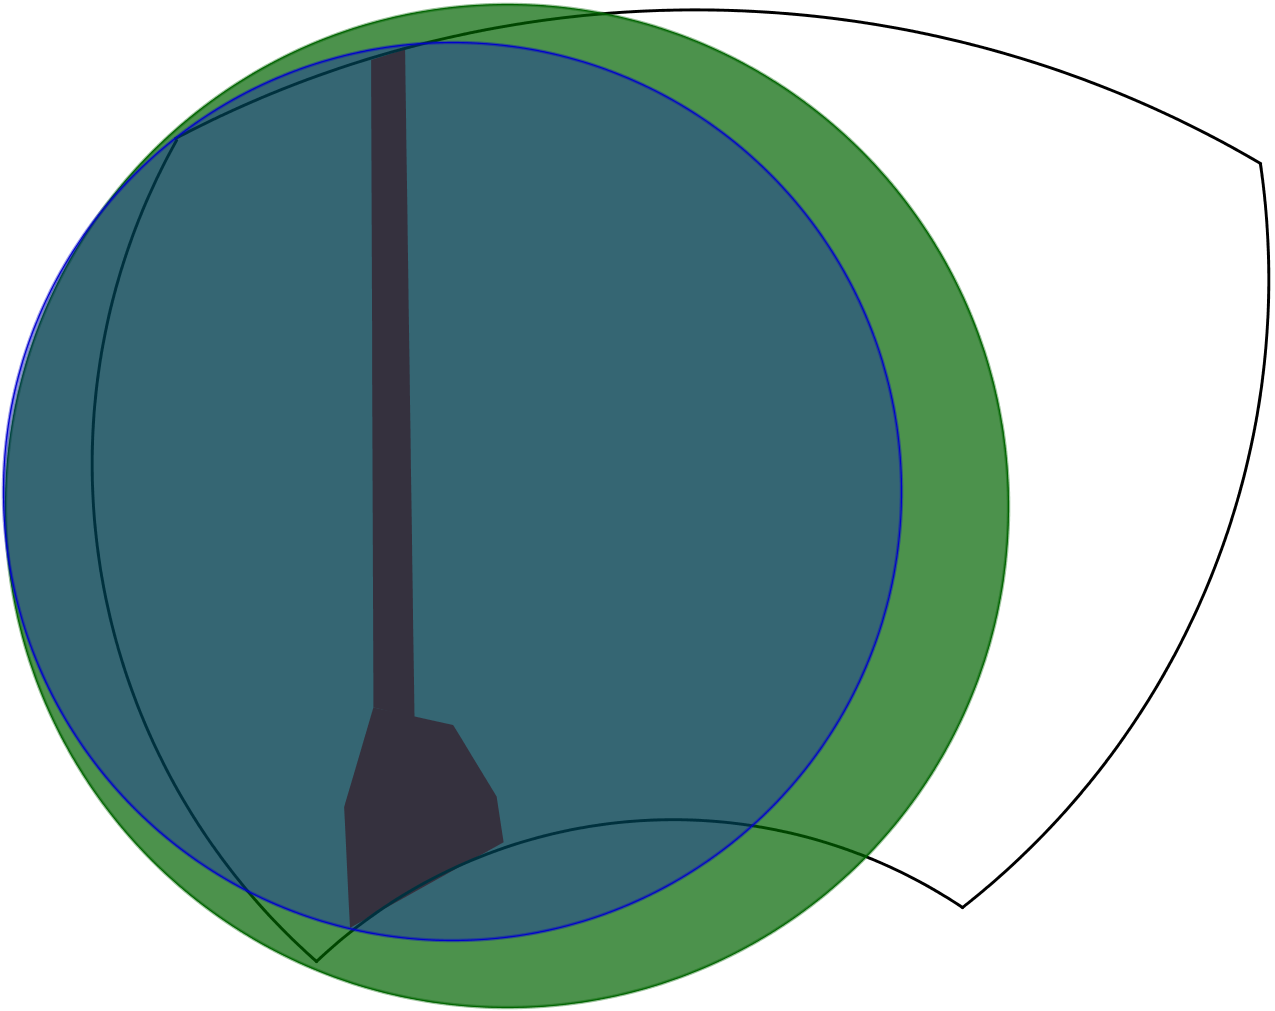
\includegraphics[width=\columnwidth]{figs/dinamica/workspaceTorques.png}
	\caption{Área em verde representa a cobertura do revestimento executada pelo
	manipulador, utilizando a abordagem dinâmica.}
	\label{fig::wdin}
\end{figure}